\documentclass[12pt, titlepage]{article}

\usepackage{booktabs}
\usepackage{tabularx}
\usepackage{float}
\usepackage{hyperref}
\usepackage[utf8]{inputenc}
\usepackage{graphicx}
\usepackage{multirow}
\hypersetup{
    colorlinks,
    citecolor=black,
    filecolor=black,
    linkcolor=red,
    urlcolor=blue
}
\usepackage[round]{natbib}

\title{SE 3XA3: Software Requirements Specification\\Ultimate Calculator}

\author{Group 15 L01
    \\ Mathew Petronilho, petronim
    \\ Jarod Rankin, rankij5
    \\ Logan Brown, brownl33
    \\ Syed Bokhari, bokhars
}

\date{\today}

%\input{../Comments}

\begin{document}

\maketitle

\pagenumbering{roman}
\tableofcontents
\listoftables
\listoffigures

\begin{table}[H]
\caption{\bf Revision History}
\begin{tabularx}{\textwidth}{p{3cm}p{2cm}X}
\toprule {\bf Date} & {\bf Version} & {\bf Notes}\\
\midrule
February 10, 2022 & 1.0 & Context, Use Cases and NFR Added\\
February 10, 2022 & 1.1 & Work Partitioning and Project Issues Added\\
February 10, 2022 & 1.2 & Project Drivers Section Added\\
February 11, 2022 & 1.3 & Constraints, Naming Conventions, Functional Requirements Added\\
February 11, 2022 & 1.4 & Symbolic Parameters, Cross Referencing\\
\bottomrule
\end{tabularx}
\end{table}

\newpage

\pagenumbering{arabic}

This document describes the requirements for the Ultimate Calculator. The template for the Software
Requirements Specification (SRS) is a subset of the Volere
template~\citep{RobertsonAndRobertson2012}.

\section{Project Drivers}

\subsection{The Purpose of the Project}
Ultimate Calculator is a multipurpose calculator that computes different and useful things that a typical calculator can not compute. This includes things such as basic arithmetic, algebraic problems, and unit conversions. The user can select what they would like to use the calculator for and enter the parameters required by the system to complete the calculation. The purpose of the project will be to redesign the outdated GUI, improve the computational algorithms currently in place, and add new features to improve the calculator functionality.

\subsection{The Stakeholders}

\subsubsection{The Client}
The clients for our project are Dr. Ashgar Bokhari, the instructor for SFWRENG 3XA3, Veerash Palanichamy and Oluwaseun Owojaiyo, the teaching assistants for lab section 1. The role of the clients is to instruct the team on what documents and deliverables need to be completed, provide help to students, and evaluate the project if it emulates the requirements found in the SRS.

\subsubsection{The Customers}
The customers of the project are students, educators, or any person who requires a multipurpose calculator. The main demographic are students, but the generality of the calculator will allow anyone to use it.
\subsubsection{Other Stakeholders}
The developers (Group 15) are stakeholders, as they are entirely involved in the creation of the project and directly influence the final outcome. Also, any person who wants to improve upon the open source code of the Ultimate Calculator are also stakeholders, as they would have interest in the success of the end product.
\subsection{Mandated Constraints}

\subsubsection{Solution Design Constraints}
\textbf{Description:} The application must operate on any personal computer machine running 
Windows, Linux or Mac OSX\\ 
\textbf{Rationale:} the user will access the application through a functioning personal computer via an operating system\\
\textbf{Fit criterion:} the application will be made to run on any personal computer running Windows, Linux or Mac OSX
\medskip\\
\\
\textbf{Description:} The application must have the necessary input sections required to compute the mathematical solution\\
\textbf{Rationale:} The user should be able to input the necessary values to compute the solution\\
\textbf{Fit criterion:} The application will include the necessary input sections required to compute the solution

\subsubsection{Partner or Collaborative Applications}
The application does not have any partner or collaborative applications. The application relies on a functioning operating system to facilitate application launch and computation.

\subsubsection{Off-the-Shelf Software}
The application does not require any Off-the-Shelf software.

\subsubsection{Anticipated Workplace Environment}
The anticipated workplace environment of the application is anywhere. The application can be run from any personal computer. Personal computers can be both portable and stationary resulting in the application being used at any location without the need for an internet connection. 

\subsubsection{Schedule Constraints}
The project will follow the predefined deadlines and due dates provided by the course instructor and the teaching assistants. The deliverables must be completed within their specific due dates and the project must be completed by April 12th, 2022. 

\subsubsection{Budget Constraints}
There is no applicable budget for this project. The cost of development tools and hardware will be out of pocket costs to the developers.

\subsubsection{Enterprise Constraints}
The application will be free to download. Any user with a functioning personal computer with an operating system will be able to access the software without the need for an internet connection.

\subsection{Naming Conventions and Terminology}
\begin{table}[H]
\centering
\footnotesize
\begin{tabular}{@{}|l|l|@{}}
\hline
{\bf Term} & {\bf Definition}  \\ \hline
Operation           & \begin{tabular}[c]{@{}l@{}}Any mathematical function that takes in one or more parameters and\\ outputs a well-defined answer\end{tabular}                                                                                                                                                           \\ \hline
Operation Type            & \begin{tabular}[c]{@{}l@{}}Class of operations with common characteristics\end{tabular} \\ \hline
Operation Section           & \begin{tabular}[c]{@{}l@{}}A window that relates to a specified operation and displays the\\ necessary parameters and result for that operation\end{tabular}  \\ \hline
Computation            & \begin{tabular}[c]{@{}l@{}}Finding the answer to a problem via mathematics\end{tabular}                                                                                                                          \\ \hline
Python            & \begin{tabular}[c]{@{}l@{}}The programming language used to develop Ultimate Calculater\end{tabular}              \\ \hline
User            & \begin{tabular}[c]{@{}l@{}}The individual interacting with the application
\end{tabular}                                                                                                            \\ \hline
Offline            & \begin{tabular}[c]{@{}l@{}}Accessing the application without the use of an internet connection\end{tabular}                                                                                                                          \\ \hline
\end{tabular}
\caption{Naming Conventions and Terminology}
\end{table}
\subsection{Relevant Facts and Assumptions}
\subsubsection{Facts}
\begin{itemize}
    \item The original repository contains approximately 3000 lines of Python code.
    \item The application has an MIT license.
\end{itemize}

\subsubsection{Assumptions}
\begin{itemize}
    \item Users have necessary equipment to run the application such as a computer, mouse, and keyboard.
    \item Users have basic knowledge of operating a computer.
    \item User have basic linguistic understanding of the English language.
    \item Users have basic knowledge of the mathematical concepts covered in the calculator section to input the values accordingly.
    \item Users have basic knowledge of calculating applications and their functionalities.
    \item Users are physically able to maneuver through the application via a mouse and keyboard.
    \item Users are visually able to maneuver through the application via mouse and keyboard.
    \item The application will be used by one user through their local machine.
\end{itemize}

\section{Functional Requirements}

\subsection{The Scope of the Work and the Product}

\subsubsection{The Context of the Work}
\begin{figure}[H]
    \centering
    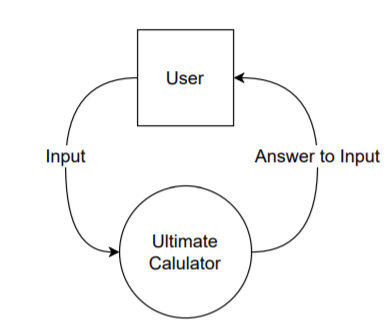
\includegraphics[scale=0.5]{Context.png}
    \caption{Context diagram for Ultimate Calculator}
    \label{fig:context}
\end{figure}
The Ultimate Calculator will be totally independent from any other external systems. There will only be a single user that interacts with the system.

\subsubsection{Work Partitioning}
\begin{table}[H]
\centering
\footnotesize
\begin{tabular}{@{}|l|l|l|l|@{}}
\hline
Event Number & Event Name               & Input                   & Output                \\ \hline
1            & Start The Application    & Keyboard                & Main Menu             \\ \hline
2            & Choose an Operation Type & Mouse Click             & Operation Type Window \\ \hline
3            & Choose Operation         & Mouse Click             & Operation Window      \\ \hline
4            & Enter a Value            & Keyboard \& Mouse Click & Value                 \\ \hline
5            & Apply the Operation      & Mouse Click             & Final Answer          \\ \hline
6            & Clear Inputs             & Mouse Click             & Empty Input           \\ \hline
7            & Close Window             & Mouse Click             & Main Menu             \\ \hline
\end{tabular}
\caption{Work Partitioning Events}
\end{table}
\begin{table}[H]
\footnotesize
\centering
\begin{tabular}{|l|l|}
\hline
Event Number & Summary                                                                                                                                                                                                                                                                                      \\ \hline
1            & \begin{tabular}[c]{@{}l@{}}The user will use their keyboard to prompt the application to start\\ from their terminal.\end{tabular}                                                                                                                                                           \\ \hline
2            & \begin{tabular}[c]{@{}l@{}}From the main menu the user will have various options of \\ operation types to click(i.e basic arithmetic, algebra, convertors, etc). \\ Once a type is chosen the user clicks on the type they desire and the \\ operation type window will appear.\end{tabular} \\ \hline
3            & \begin{tabular}[c]{@{}l@{}}From the main menu the user will have various options of\\  operation types to click(i.e basic arithmetic, algebra, convertors, etc).\\ Once a type is chosen the user clicks on the type they desire and the \\ operation type window will appear.\end{tabular}  \\ \hline
4            & \begin{tabular}[c]{@{}l@{}}From the operation window the user will click on the input box they \\ desire and type in their inputs with their keyboard.\end{tabular}                                                                                                                          \\ \hline
5            & \begin{tabular}[c]{@{}l@{}}From the operation window the user can complete an operation\\ and find a final answer. The user must have the inputs filled in\\ and if they are they will click a calculate button. The user will be shown \\ the answer they desire.\end{tabular}              \\ \hline
6            & \begin{tabular}[c]{@{}l@{}}In the operation window the user can click the clear button found\\ in the current window to clear all values they have previously input.\end{tabular}                                                                                                            \\ \hline
7            & \begin{tabular}[c]{@{}l@{}}If a user chooses to close a window or close the application they can \\ select the X button found in the top right corner.\end{tabular}                                                                                                                          \\ \hline
\end{tabular}
\caption{Work Partitioning Events Summaries}
\end{table}
\subsubsection{Individual Product Use Cases}
\begin{figure}[H]
    \centering
    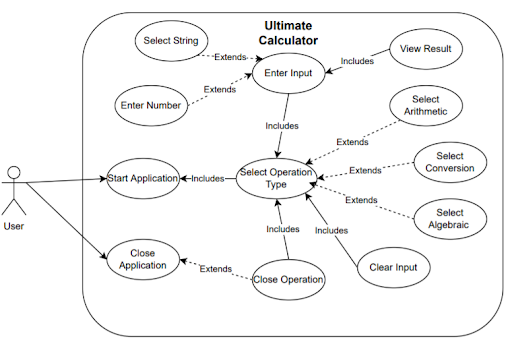
\includegraphics[scale=0.7]{UseCase.png}
    \caption{Use Case diagram for Ultimate Calculator}
    \label{fig:usecase}
\end{figure}

\begin{table}[H]
\centering
\begin{tabular}{|l|l|l|}
\hline
Actor & Actors Goal                                                    & Use Case                \\ \hline
User  & To open the application to begin computing.                    & UC1 - Start Application \\ \hline
User  & To perform a specific computation.                             & UC2 - Select Operation  \\ \hline
User  & \begin{tabular}[c]{@{}l@{}}To enter the necessary parameters \\ for the desired calculation.\end{tabular} & UC3 - Enter Input       \\ \hline
User  & To see the answer of the computation.                          & UC4 - View Result       \\ \hline
User  & To remove previous inputs.                                     & UC5 - Clear Input       \\ \hline
User  & To stop using a specific operation.                            & UC6 - Close Operation   \\ \hline
User  & To stop using the application.                                 & UC7 - Close Application \\ \hline
\end{tabular}
\caption{Brief Summary of Use Cases}
\label{tab:usecase}
\end{table}

Figure \ref{fig:usecase} illustrates several ways in which the user can interact with our system and the possible actions that they would want to perform. An overview of the main use cases can be seen in Table \ref{tab:usecase}.

\subsection{Functional Requirements}

\begin{enumerate}

\item [FR1] The system must display all operation types of the calculator upon the start of the application.
\item [FR2] The system must have at least $\hyperlink{minop}{MIN\_UNIQUE\_OP}$ unique operation types.
\item [FR3] The system must have a minimum of $\hyperlink{minsec}{MIN\_OP\_SECTION}$ operation sections for every operation type.
\item [FR4] The system must start users at the main menu.
\item [FR5] The system must initialize all input parameters for an operation to be empty upon user selection of that operation.
\item [FR6] The system must display a calculate button in every operation section.
\item [FR7] The system shall let the user compute multiple operations synchronously.
\item [FR8] The system must provide users with a way of entering input parameters.
\item [FR9] The system must have a minimum of $\hyperlink{minin}{MIN\_INPUT}$ input for every operation section.
\item [FR10] The system must display the input that the user has provided.
\item [FR11] The system must tell the user if their inputs result in mathematical errors such as a division by 0 error.
\item [FR12] The system must prevent users from entering non-valid input types and provide a warning.
\item [FR13] The system must notify user if the necessary input fields are not populated.
\item [FR14] The system must produce mathematically correct results based on well known arithmetic rules.
\item [FR15] The system must display the results of a calculation to the user.
\item [FR16] The system must allow the user to clear input.
\item [FR17] The system must be able to clear all user input in the selected operation.
\item [FR18] The system must allow the user to close an operation section.
\item [FR19] The system must allow the user to close the main menu at any time.
\item [FR20] The system must close all operation sections upon the closing of the main menu.
\item [FR21] The system must prompt the user with a confirmation window when they choose to close the main menu.

\end{enumerate}

\section{Non-functional Requirements}

\subsection{Look and Feel Requirements}
\subsubsection*{Requirement NF1:}
\begin{itemize}
  \item \textbf{Description:} The main menu must resemble a standard calculator with various additions.
  \item \textbf{Rationale:} Keeps the appearance in line with the context of the application.
  \item \textbf{Fit Criterion:} The main menu has similar appearance traits to a real calculator such as an output screen and buttons.
\end{itemize}

\subsubsection*{Requirement NF2:}
\begin{itemize}
  \item \textbf{Description:} All sections of the application must be similar in appearance.
  \item \textbf{Rationale:} This will make the application look more cohesive and professional.
  \item \textbf{Fit Criterion:} Font type, sizing, and colour, along with background colours will all be consistent throughout the application.
\end{itemize}



\subsection{Usability and Humanity Requirements}
\subsubsection*{Requirement NF3:}
\begin{itemize}
  \item \textbf{Description:} All operation sections shall be easy to access.
  \item \textbf{Rationale:} The user wants to get to a specific operation section quickly and efficiently.
  \item \textbf{Fit Criterion:} The user should be able to access a specific operation section within $\hyperlink{maxclicks}{MAX\_NAVIGATION\_CLICKS}$ mouse clicks.
\end{itemize}

\subsubsection*{Requirement NF4:}
\begin{itemize}
  \item \textbf{Description:} Maneuvering through the menus shall be simple.
  \item \textbf{Rationale:} The user wants to be able to locate what they want intuitively.
  \item \textbf{Fit Criterion:} All navigation buttons will be specifically labeled or have descriptive images on them.
\end{itemize}


\subsection{Performance Requirements}
\subsubsection*{Requirement NF5:}
\begin{itemize}
  \item \textbf{Description:} The transitions from each individual menu should be a smooth and fluid process.
  \item \textbf{Rationale:} This is will improve the experience of the users of the application.
  \item \textbf{Fit Criterion:} A menu should appear in a maximum of $\hyperlink{maxresponse}{MAX\_RESPONSE\_TIME}$ seconds after it has been prompted.
\end{itemize}

\subsubsection*{Requirement NF6:}
\begin{itemize}
  \item \textbf{Description:} The system must display the results of an operation quickly.
  \item \textbf{Rationale:} If a calculation takes too long the calculator will not be viable.
  \item \textbf{Fit Criterion:} The result must be displayed by the system in less than $\hyperlink{maxresponse}{MAX\_RESPONSE\_TIME}$ seconds from once the calculate button has been selected.
\end{itemize}

\subsubsection*{Requirement NF7:}
\begin{itemize}
  \item \textbf{Description:} The system shall display a maximum of $\hyperlink{maxsf}{MAX\_SIG\_FIGS}$ significant digits for any calculation result.
  \item \textbf{Rationale:} The GUI only has a certain amount of space for displaying answers, so a number with too many significant digits may result in an overflow of numbers off the GUI.
  \item \textbf{Fit Criterion:} A maximum of $\hyperlink{maxsf}{MAX\_SIG\_FIGS}$ significant digits is displayed by the system.
\end{itemize}


\subsection{Operational and Environmental Requirements}
\subsubsection*{Requirement NF8:}
\begin{itemize}
  \item \textbf{Description:} The system must work without the use of an internet connection.
  \item \textbf{Rationale:} To allow the user to use the application anytime and anywhere.
  \item \textbf{Fit Criterion:} The application works without access to the internet.
\end{itemize}


\subsection{Maintainability and Support Requirements}
\subsubsection*{Requirement NF9:}
\begin{itemize}
  \item \textbf{Description:} The product must be made open source where anyone can submit bugs and issues.
  \item \textbf{Rationale:} This will allow for any changes or issues to be easily tracked.
  \item \textbf{Fit Criterion:} The product is open source on a website such as GitLab or GitHub.
\end{itemize}

\subsubsection*{Requirement NF10:}
\begin{itemize}
  \item \textbf{Description:} The system must allow new operation types to be easily added.
  \item \textbf{Rationale:} If updates are to be made in the future, this will be necessary.
  \item \textbf{Fit Criterion:} The code is modular and exhibits low coupling and high cohesion.
\end{itemize}

\subsection{Security Requirements}
N/A

\subsection{Cultural Requirements}
N/A
\subsection{Legal Requirements}
N/A
\subsection{Health and Safety Requirements}
N/A

\section{Project Issues}

\subsection{Open Issues}
There were not any issues in the implementation of the Ultimate Calculator. The downloadable executable file launches the console based calculator but the GUI requires additional setup to work.
\subsection{Off-the-Shelf Solutions}
Symbolab is the best known answer engine found on the internet, but it is not an open source project like our Ultimate Calculator. Symbolab contains several advantages that allow the user to do various calculations most open source calculators can not do. Yet, Symbolab is less convenient as it can not function without the use of the internet. Another off-the-shelf solution would be a handheld calculator. The handheld calculator can function without the use of the internet but it can not do the advanced calculations that the Ultimate Calculator can.
\subsection{New Problems}
Additional operations such as matrix manipulation and GPA calculation will be added. A new and improved GUI will also be a part of the project.
\subsection{Tasks}
\begin{enumerate}
    \item Design templates of the new GUI look for all sections of the application.
    \item Modularize the source code further.
    \item Make original source code more robust when it comes to erroneous inputs.
    \item Implement the new GUI designs within our application.
    \item Implement new functionality and operations for the calculator.
    \item Implement GUI designs for the new operations within our application.
    \item Complete all course deliverables on time.
\end{enumerate}
\subsection{Migration to the New Product}
The new Ultimate Calculator will use elements of the previous implementation such as backend calculations, but a new GUI will be used.
\subsection{Risks}
There is little to no risk with this project as the mathematics underlying the calculator are already well established and well documented. The risks of the program include imprecise answers to calculations and unexpected errors such as divide by zero. These risks will be mitigated by thorough testing.
\subsection{Costs}
There is no monetary cost associated with the development of the application. The development of the application is estimated to consume a time cost and requires prerequisite software and hardware that the developers must provide for themselves.
\subsection{User Documentation and Training}
\subsubsection{User Documentation}
There will be a README file available that guides the user through the installation process.
\subsubsection{Training}
No training is required to use the Ultimate Calculator application. The selections are intuitive and a basic understanding of how to input values is required.
\subsection{Waiting Room}
If time is found for additional implementations these ideas would be considered.
\begin{enumerate}
    \item Integral Calculator
    \item Derivative Calculator
    \item Graphing Calculator
\end{enumerate}
\subsection{Ideas for Solutions}
N/A
\bibliographystyle{plainnat}

\bibliography{SRS}

\newpage

\section{Appendix}

This section has been added to the Volere template.

\subsection{Symbolic Parameters}
$\hypertarget{maxresponse}{MAX\_RESPONSE\_TIME}$ = 2\\
$\hypertarget{maxclicks}{MAX\_NAVIGATION\_CLICKS}$ = 2\\
$\hypertarget{maxsf}{MAX\_SIG\_FIGS}$ = 10\\
$\hypertarget{minop}{MIN\_UNIQUE\_OP}$ = 5\\
$\hypertarget{minsec}{MIN\_OP\_SECTION}$ = 3\\
$\hypertarget{minin}{MIN\_INPUT}$ = 1\\



\end{document}